
\documentclass[11pt]{report}
\usepackage{graphicx}
\usepackage{url}
\usepackage{amsmath}
\usepackage{verbatim}
\title{TDT4255 Assignment 3}
\author{Knut Halvor Skrede \& Ole Magnus Ruud}
\begin{document}
\maketitle
\clearpage


\section*{Abstract/Summary}
        
% Lab-report presents documentation of your work which was done during the exercise. 
% It is important
% that the reader can understand what the group has done and how it came to the solution.
% In short, abstract should contain overview of:
% – what the task of the exercise was
% – how it was solved
% – what works
% – what does not work
% – if something extra was done by the group
% – if something should have been done in another way

The task was to implement a simple pipelined CPU. A top level architecture 
was proposed in the assignment text, we chose to implement the CPU in this way. 
The CPU should load instructions from memory and execute them. 
A program counter will be used to walk through the 
instructions. A BNZ (branch if not zero) instruction can also be used, this 
instruction will load the program counter with a given address if the zero flag
was deasserted from the previous ALU instruction. Additionally the CPU should implement a 
LDI (load immediate) instruction that loads the the register with a value. 
The CPU should also implement LOAD and STORE instructions to operate on memory.
We implemented 3 seperate test programs to be simulated and run on the implemented
fpga. These programs were made to test if the CPU operated correctly under different
situations.

\section*{Introduction}

% Present what the task within the exercise is and what challenges it
% gives.  For example, which kind of program has to be written and
% which hardware has to be used.  Short introduction to how the group
% has solved this task.  It is important that what has been
% accomplished is clearly presented.  If there is something in the
% exercise what has not been completed or what does not function as it
% should, it should also be described.  If applicable, write on the
% motivation and solution(s) for extra functionality which the group
% has set in.

The task of this assignment was to expand the design from the previous
assignment with pipelining and a data storage memory, and make it work
on Nalle. To do this, it
was necessary to add registers between each pipelining stage containing
all information and control signals needed for later stages. It was also
necessary to take dependancy hazards into account by writing back results
to where it is needed in the earlier pipelining stages. 

We used the suggested solution in the exercise as a starting point, 
especially the architecture illustration which we have included in 
Figure \ref{fig:architecture}.
  
\begin{figure}[htbp]
    \centering
    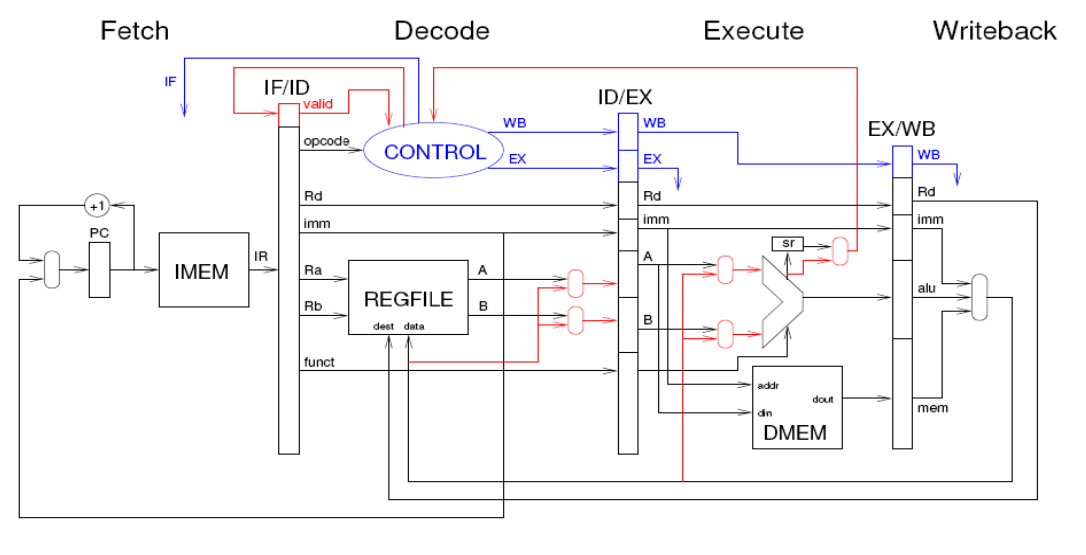
\includegraphics[width=.95\linewidth]{toplevel.png} 
    \caption{Pipelined CPU architecture from the assignment text}
    \label{fig:architecture}
  \end{figure}



% Present concisely an outline of how the task was solved.  This is
% the place to write in greater detail about how the group was
% developing ideas for achieving solution.  Add an outline of, for
% example, how hardware is built up and how it functions.  It is
% advised to use concise and clear flow diagrams, UML or block
% diagram.  All code should be delivered in a separate file. It is
% important that documentation contains enough description of the
% program so that the reader can understand how the program works and
% what files with the source code are attached. Write about how the
% group has come to the solution, what tests were used to ensure that
% the program runs as it should, for example, what documentation the
% group has used, possibly some additional sources which were helpful
% to do the exercise.  Remember that documentation is a part of the
% grade. So, it is not enough to have a brilliant solution if the
% reader can't understand how it is meant to work.

\section*{Design}

% Write somthing about instruction format, implemented functions. Data sizes and so on.
% Describe computation flow, what happens at each stage
\subsection*{Instruction format}

\begin{table}[h]
  \centering
  \begin{tabular}{|l|l|l|l|l|l|l|l|}
    \hline
    Name: 		&	Opcode		&	unused	&	funct	&	Imm		&	Rd		&	Ra	&	Rb	\\\hline
    Bits: 		&	31-29		&	28-24	&	23-20	&	19-12	&	11-8	&	7-4	&	3-0	\\\hline
  \end{tabular}
  \caption{Instruction set format}
  \label{tab:instformat}
\end{table}

As our instruction format we decided to use a slightly modified version of the
suggested format from assignment 2, shown in table \ref{tab:instformat}. The only
difference is that Ra and Rb are swapped. Following is a description of the different
fields.

\begin{description}
\item[Opcode] - Used to determine the control signals in the cpu given different instructions.	
\item[Funct] - Used for choosing the ALU instruction.
\item[Immediate] - Used in different instructions as a constant value.
\item[Rd] - Number of the register which will be written
\item[Ra] - Number of operand register A
\item[Rb] - Number of operand register B
\end{description}



\subsection*{Implemented functions}

The cpu implements the following functions, the opcodes and funct 
codes are defined in table \ref{tab:opcodes} and table \ref{tab:functcodes}:
\begin{enumerate}
  \item BNZ: Branch not zero, executes an absolute jump to the address given by
the immediate value of the instruction if the zero flag in the status register is deasserted.
  \item LDI: Load immediate, Loads a register with the immediate value of the instruction.
  \item LOAD: Loads a register with a value from memory at address given by immediate.
  \item STORE: Stores a value from register to memory at address given by immediate.
  \item ALU Instructions:
  \begin{enumerate}
    \item MOVE: Moves a register value to a target register
    \item AND: Performs a bitwise and on the registers and stores to a target register.
    \item ADD: Adds the values from the registers and stores to a target register
  \end{enumerate}
\end{enumerate}

\begin{table}[h]
  \centering
  \begin{tabular}{|l|l|l|}
    \hline
    Name&Opcode&Comment \\
    \hline
    ALU\_INST	&001	&Writes alu result to register\\
    BNZ			&011	&Loads pc register if zero flag is not set\\
    LDI			&010	&Loads register with value\\
    LOAD		&110	&Writes register Ra to memory at address given by immediate\\
    STORE		&100	&Loads register Rd with memory at address given by immediate\\
    \hline
  \end{tabular}
  \caption{Instruction set for the CPU, not including the alu functionality}
  \label{tab:opcodes}
\end{table}

\begin{table}[h]
  \centering
  \begin{tabular}{|l|l|l|}
    \hline
    Name&Funct&Comment \\
    \hline
    MOVE	&0000	& sets output of ALU out to input A\\
    AND		&0001	& Bitwise AND of input A and B\\
    ADD		&0111	& Arithmetic ADD of input A and B\\
    \hline
  \end{tabular}
  \caption{Function set for the ALU}
  \label{tab:functcodes}
\end{table}


\subsection*{Processor Operation}
We will here describe the basic flow of operations for an instruction
through our processor architecture stage by stage without hazards handling.
The additions to handle hazards will be described in the hazards section.
The stages correspond to the stages of Figure \ref{fig:architecture}.

\subsubsection*{Instruction fetch}


Instructions starts out by being fetched based on the program counter from the
instruction memory to the IF/ID register. This is the complete basic operation of the 
instruction fetch stage.
\subsubsection*{Decode}

In the decode stage the most basic action is the forwarding of the Rd, Immediate and
the function field to the ID/EX register. The Ra and Rb fields are sent to the regfile, 
and the corresponding outputs are written to the ID/EX A and B field. 
The immediate field is also connected to the data memory read address, as this value
needs to be read on a rising edge because of the delivered memory implementation.

Based on the opcode of the instruction, control has to write several control signals 
to the ID/EX register. These are divided into control signals for the Execute stage
and control signals for the writeback stage.

The execute control signals are memory write enable, which is set for memory write instructions,
and status write enable, which is set for ALU instructions.

The writeback control signals are source select and register write enable. 
The source select is the control signal for the register input selector,
which is set to alu output for alu operations, memory output 
for load instructions and immediate for load immediate. 
The register write enable is set for all instructions resulting in a register write.

\subsubsection*{Execute}

In the execute stage the Rd, immediate and writeback control signal fields are 
forwarded from ID/EX to EX/WB. 

The ALU combinatorially computes an output value based on
the A, B and function fields of the ID/EX register, and stores it in an ALU field in
the EX/WB register. The output from the ALU status is sent to the Status register along
with the status register write signal from the ID/EX register which decides if the 
register is written.

The immediate value from the Decode stage has now been caught 
by the Data memory, and the value stored at this address is written to the memory field
of the EX/WB register. The immediate, A and memory write enable fields of the ID/EX register
are sent to the write address, write data and write enable inputs of the data memory,
respectively. If the write enable is asserted, the data is written.

\subsubsection*{Writeback}

In the writeback stage the register file is written if the register write enable
signal of the EX/WB register is asserted. The value written is selected with a register
input mux based on the source select signal in the EX/WB register with all the data fields
of EX/WB as inputs. The register destination is decided by the propagated Rd field of the
EX/WB register.



\subsection*{Hazards handling}

A big part of this assignment was handling the various forms of Hazards 
encountered in pipelining processors. In our architecture there are two potential
types of hazards, data hazards and control hazards. The data hazards occur when there 
are data dependencies between closely following instructions, resulting in the
early instructions not being able to write their result before the same result is 
supposed to be read by a following instruction. The control hazard occur when a branch
is being taken, but the instruction following the branch is already inserted in the pipeline,
even though it is not supposed to be executed.

We will now describe how both of these hazards are being handled in our architecture.

\subsubsection*{Control hazard handling}

To handle the control hazards we have done as the assignment text proposes, and included
a valid bit for the IF/ID register. This valid bit is written by the control unit in the
instruction fetch stage. Checking if the current opcode 
corresponds to a BNZ instruction and that the status register is not zero
is enough to know if the branch is being taken, and so the valid bit can be deasserted. 
When the control unit checks the valid bit the next cycle, it knows it is dealing with an 
invalid operation and can resolve this by deasserting all write enable signals in the 
ID/EX register.

\subsubsection*{Data hazard handling}

As figure \ref{fig:architecture}
illustrates, the register file is not written until the end of the 
writeback stage, but at this stage there are already two following instructions that
have performed or are performing their register reads, the one in the execute stage, 
and the one in the 
decode stage. This means that if these following instructions share a source register
number with the first instruction's write register number, the data read will be wrong. 

The solution to this problem is to bypass the register file, by connecting the output
from the register input muxer to four different muxes, one for each input value in both
the decode and execute stage. These are the red muxes in figure \ref{fig:architecture}.
We will get back to the final red mux by the status register. 

The two muxes in the
decode stage are directly controlled by the control unit, while the two control signals 
for the execute stage has to be written to the ID/EX pipeline register to be used in the 
execute stage. One addition to the figure, is that the output from the A operand muxer in 
the execute stage also is connected to the write data input of the data memory, as the
same data hazard is valid for memory writes. The control signals are asserted 
according to table \ref{tab:hazmuxes}. 

In addition, the muxes are not asserted when 
the write destination registers are register 0, 
as this is constant Zero, and when the register write enable signals are deasserted.
Notice that if for example Ra of an instruction is written by both preceeding 
instructions, the closest one takes precedence, as the writeback value in the
execute stage overwrites the one from the decode stage. Also, any number of the 
muxer controls may be asserted, as in the extreme case where both preceeding instructions
write the same register, and both read registers of the current instructions are the same.

\begin{table}[htbp]
  \centering
  \begin{tabular}{|l|l|}
    \hline
    Condition&Asserted multiplexor \\
    \hline
    EX/WB Rd = IF/ID Ra	& Decode mux A\\
    EX/WB Rd = IF/ID Rb	& Decode mux B\\
    ID/EX Rd = IF/ID Ra	& Execute mux A\\
    ID/EX Rd = IF/ID Rb	& Execute mux B\\
    \hline
    
  \end{tabular}
  \caption{Control of the data hazard multiplexors}
  \label{tab:hazmuxes}
\end{table}


The last hazard is the status register read by our branch if not zero instruction.
If the instruction preceeding a branch instruction is an ALU instruction, meaning it
is setting the status register, this status will not be ready in the status register
until after the branch evaluation has been performed, possibly resulting in an
erroneous branch. This is solved with the status muxer mentioned earlier, and is the 
red muxer by the status register in figure \ref{fig:architecture}.
This muxer is simply controlled by the status write enable signal itself, directing the
newest status to the control unit.


\section*{Approach}

%We started by making skeleton modules for all the components, mapping
%the signals between them. After that we implemented the simplest
%components. To make sure nothing was wrong before writing the more
%difficult components, we wrote simple testbenches for them. We then
%proceeded to implement the control unit, which we considered to be the
%most challenging component. We then wrote a more general testbench for
%the CPU, and after debugging and figuring out some timing issues, we
%tested it on nalle running a program calculating fibonacci numbers.

Our approach to the problem in this excercise was to construct all the 
modules described in figure \ref{fig:architecture}, starting with the simplest.  %DIAGRAM!
This included the writeback muxes between the register file and the id/ex
pipeline register and the writeback muxes between the id/ex pipeline 
register and the ALU and data memory as we felt confident we were going 
to get the hazards handling working. 
Some of the modules like the program counter and status register 
we reused from the previous assignments.

When the muxes were finished, we had a good indication on what control
signals would be needed for all the pipelining stages, and so we could 
implement the pipelining registers with all of these control signals.

The final and most difficult component we implemented was the control
module setting all the control signals. When we thought we had it right
everything was sewed together and we could test it with a testbench
from the previous assignment. After some debugging in Modelsim we had 
a working architecture.

\subsection*{Implementation}

Our implementation consists of a cpu component composed of
the following components ordered by their appearance 
in the pipelining stages as shown in figure \ref{fig:archnumbered}:
	
\begin{enumerate}
\item Program counter.
\item Instruction memory.
\item IF/ID pipeline register.
\item Control unit.
\item Register file.
\item Register to ID/EX muxes.
\item ID/EX pipeline register.
\item ID/EX to ALU and data memory muxes.
\item ALU.
\item Status Register
\item Data memory.
\item EX/WB pipeline register.
\item Register input mux.
\end{enumerate}

\begin{figure}[htbp]
  \centering
  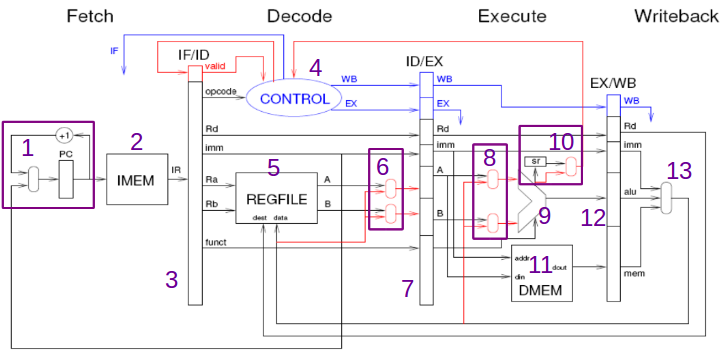
\includegraphics[width=0.95\linewidth]{toplevelmarked.png} \\
  \caption{Architecture with numbered components}
  \label{fig:archnumbered}
\end{figure}
	
We will now describe the implementations of these components.
\subsubsection*{Program Counter (pc.vhd)}
%The program counter is initiated to 0 on reset and is updated every control cycle
%with either an increment or an immediate value from the instruction. 
%We discussed using a relative jump instead of just loading a value, 
%but decided to drop this as there is no need for relative jumps when running 
%single programs and we have full control of memory.
The program counter is the same one used in the previous assignment. 
It is a counter with an initial value of 0 after reset, with a built in
mux choosing between a provided immediate value, and the incrementation of
the current value. It also takes in a write enable that is not needed in
the current architecture, but that would be if we decided to expand the 
instruction set in the future.

\subsubsection*{Instruction memory (mem.vhd)}
The instruction memory is an instantiation of the provided memory component
with word size generic set to 32(our instruction size). It takes in
output from the program counter and fetches the instruction at the provided
address for the rest of the cpu.
\subsubsection*{IF/ID pipeline register (if\_id\_reg.vhd)}
Since the instruction is stored on the output register of the instruction memory,
the IF/ID pipeline register component is actually just an abstraction of this, sending 
most of its input straight through, and only registering the valid bit, provided by
the control module. For simplicity we created a record holding all the required fields
to use as output from this component. We did this for the other pipeline registers
also, and they are all declared in the package.vhd file.

\subsubsection*{Control Unit (control.vhd)}

The control unit is the most complex component in our design, as all the control
signals in the decode stage is set here, as well as the future control signals for
the execute and writeback stage that must be written to the ID/EX pipeline register.
The component is purely combinatorial, with outputs based on the current instruction in the
IF/ID register and some fields in the other pipeline registers to handle hazards as
described in the hazard section of the report. It's function is described further in the 
earlier processor operation section.

\subsubsection*{Register file (regfile.vhd)}
The register file is an instantiation of the delivered register file, with 
2 combinatorial read adresses with corresponding 8 bit outputs, and one sequential
write address and 8 bit data port.

\subsubsection*{Register to ID/EX muxes (id\_operand\_mux.vhd)}
Based on two control signals from the control unit, this double mux combinatorially
decides the input of the two operand fields of the ID/EX register. It can 
either be from the register or the writeback signal from the writeback stage.

\subsubsection*{ID/EX pipeline register (id\_ex\_reg.vhd)}
This is a simple sequentially written register. The contents are described in the 
processor operation and hazards handling sections, and is defined as a record in package.vhd. 
\subsubsection*{ID/EX to ALU and data memory muxes (ex\_operand\_mux.vhd)}
This component works the same way as the Register to ID/EX mux, but the source of the 
mux control signals is the ex field of the ID/EX register, and the ouput is connected
to the ALU and Data memory data input.

\subsubsection*{ALU (alu.vhd)}
The ALU used is the one from the support files. It is an 8-bit ALU.
\subsubsection*{Status Register (sr.vhd)}
We use our Status Register implementation from the previous assignment, but have
built in the writeback mux to be controlled by the write status register signal.
When the status write signal is asserted, the mux will also choose the current 
status signal from the ALU, even before it is written to the register.
\subsubsection*{Data Memory (mem.vhd)}
As with the Instruction memory, this is an instantiation of the handed out memory
module, only used for data. This implies an 8-bit width. Because it needs the read address
on the rising edge, we had to connect the read address port to the immediate value of the
if/id register.
\subsubsection*{EX/WB pipeline register (ex\_wb\_reg.vhd)}
As with ID/EX this is just a simple register. Fields are described in the design section.
\subsubsection*{Register input mux (regfile\_mux.vhd)}
Our last component is the muxer choosing what value of the EX/WB register to send to the
register file. 
%The status register is just a register with a write enable, and the register 
%multiplexer is just a mux placed in a component to clean up our CPU code.  


\subsection*{Testing}

\subsubsection*{Pipeline flushing test}

This program tests if the instruction after a branch is successfully flushed.
The program segment loads two values, 246 and 1. It then adds 1 to 246 and
branches back to the add instruction until it reaches 255 and then overflows
to 0. After the overflow add the branch should not be taken and the next instruction
should be executed. If it fails, the register holding 1 will be loaded with 10
and the program will not perform as expected. This program is included as a bitfile
('test\_program\_1.txt') and explained in table \ref{tab:program1table}. It is also the 
program being run in 'cpu\_testbench.vhd'.
The waveform of this test can be seen in figure \ref{fig:program1wave}

\begin{table}[htbp]
  \centering
  \begin{tabular}{|c|c|c|c|c|c|c|}
    \hline
    Line Nr &	Opcode		&	funct	&	Imm	&	Rd	&	Ra	&	Rb	\\\hline
    	0	&	LDI			&			&	246	&	1	&		&		\\\hline
    	1	&	LDI			&			&	1	&	2	&		&		\\\hline
    	2	&	ALU\_INST	&	ADD		&		&	1	&	2	&	1	\\\hline
    	3	&	BNZ			&			&	2	&		&		&		\\\hline
    	4	&	LDI			&			&	10	&	2	&		&		\\\hline
  \end{tabular}
  \caption{Program to test branching}
  \label{tab:program1table}
\end{table}

\begin{figure}
  \centering
  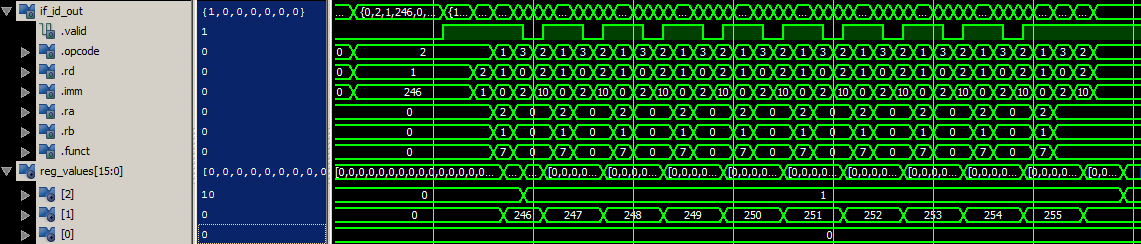
\includegraphics[width=.95\linewidth]{test1.png} \\
  \caption{This figure shows the waveform from the testbench, 
  most of the register signals has been removed, this is because they are not beeing used.}
  \label{fig:program1wave}
\end{figure}


\subsubsection*{Data dependency test}

This program tests if the dataforwarding is successfull. The part after 'Test 1' tests data forwarding
from the writeback- to the execute-stage. The part after 'Test 2' tests data forwarding from the
writeback- to the decode-stage. It is included as a bitfile ('test\_program\_2.txt') and explained
in table \ref{tab:program2table}. It is also the program being run in 'cpu\_testbench2.vhd'.
The waveform of this test can be seen in figure \ref{fig:program2wave}

\begin{table}[htbp]
  \centering
  \begin{tabular}{|c|c|c|c|c|c|c|}
    \hline
    Line Nr &	Opcode		&	funct	&	Imm	&	Rd	&	Ra	&	Rb	\\\hline
    	0	&	LDI			&			&	18	&	1	&		&		\\\hline
    	1	&	LDI			&			&	2	&	2	&		&		\\\hline
	\multicolumn{7}{|c|}{Test 1: Dataforwarding from writeback- to execute-stage (one-stage forwarding)}\\\hline
    	2	&	ALU\_INST	&	ADD		&		&	1	&	2	&	1	\\\hline
    	3	&	ALU\_INST	&	ADD		&		&	1	&	2	&	1	\\\hline
    	4	&	ALU\_INST	&	ADD		&		&	1	&	2	&	1	\\\hline
	\multicolumn{7}{|c|}{Test 2: Dataforwarding from writeback- to decode-stage (two-stage forwarding)}\\\hline
    	5	&	ALU\_INST	&	ADD		&		&	1	&	2	&	1	\\\hline
    	6	&	ALU\_INST	&	ADD		&		&	1	&	2	&	2	\\\hline
    	7	&	ALU\_INST	&	ADD		&		&	1	&	2	&	1	\\\hline
  \end{tabular}
  \caption{Program to test data forwarding}
  \label{tab:program2table}
\end{table}

\begin{figure}
  \centering
  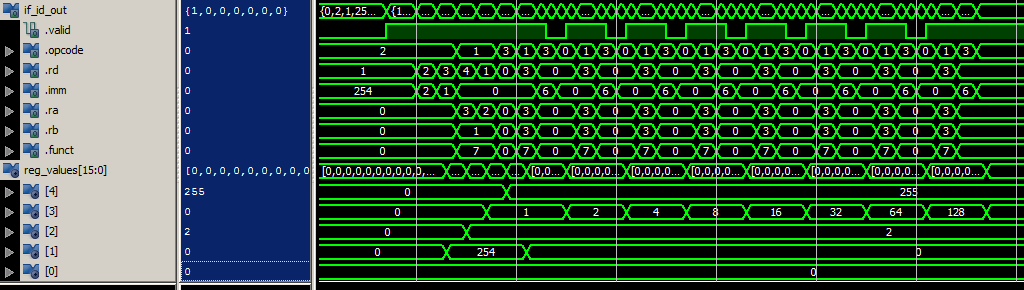
\includegraphics[width=.95\linewidth]{test3.png} \\
  \caption{This figure shows the waveform from the testbench, 
  most of the register signals has been removed, this is because they are not beeing used.}
  \label{fig:program2wave}
\end{figure}

\subsubsection*{Status register test}

This program test if the statusregister is successfully forwarded.
It first loads 254 to register 1, 2 to register 2 and 1 to register 3.
It then adds 254 and 1 and writes it to register 4, the result should be
255. It then adds 2 to 254, this operations should overflow and result in zero,
resulting in the following branch instruction not to be taken. The instructions
following this test should count upwards in the power of 2 until it overflows
and stops. This program is included as a bitfile ('test\_program\_3.vhd') and
explained in table \ref{tab:program3table}. It is also the program being run in 'cpu\_testbench3.vhd'.
The waveform of this test can be seen in figure \ref{fig:program3wave}

\begin{table}[htbp]
  \centering
  \begin{tabular}{|c|c|c|c|c|c|c|}
    \hline
    Line Nr &	Opcode		&	funct	&	Imm	&	Rd	&	Ra	&	Rb	\\\hline
    	0	&	LDI			&			&	254	&	1	&		&		\\\hline
    	1	&	LDI			&			&	2	&	2	&		&		\\\hline
    	2	&	LDI			&			&	1	&	3	&		&		\\\hline
    	3	&	ALU\_INST	&	ADD		&		&	4	&	3	&	1	\\\hline
    	4	&	ALU\_INST	&	ADD		&		&	1	&	2	&	1	\\\hline
    	5	&	BNZ			&			&	0	&		&		&		\\\hline
    	6	&	ALU\_INST	&	ADD		&		&	3	&	3	&	3	\\\hline
    	7	&	BNZ			&			&	6	&		&		&		\\\hline

  \end{tabular}
  \caption{Program to test data forwarding}
  \label{tab:program3table}
\end{table}

\begin{figure}
  \centering
  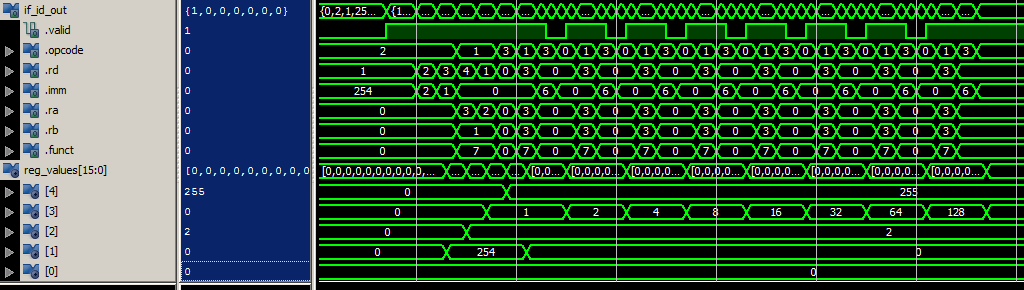
\includegraphics[width=.95\linewidth]{test3.png} \\
  \caption{This figure shows the waveform from the testbench, 
  most of the register signals has been removed, this is because they are not beeing used.}
  \label{fig:program3wave}
\end{figure}

\subsubsection*{Comparison to the multicycle CPU}

The fibonacci program described in table \ref{tab:fibonacci} simply loads the value 1
to register 1 and 2. It then adds registers 1 and 2 to register 1 and then it adds
register 2 and 1 to register 2 and branches back to the first add instruction. The 
branch instruction used is BNZ (branch not zero), since the second ADD instruction
will never result in 0 the program will continue forever. We tested the program on
the multicycle cpu and the pipelined cpu by singlestepping through the program and
counting the steps required to get to fibonacci number 233 ( E9 in hex ). The result
was that the multicycle cpu used 36 steps, and the pipelined cpu used 26. This is a
significant increase in performance. This program may however be a poor representation
of the difference in performance as there are alot of branches being taken.

\begin{table}[htbp]
  \centering
  \begin{tabular}{|c|c|c|c|c|c|c|}
    \hline
    Line Nr &	Opcode		&	funct	&	Imm	&	Rd	&	Ra	&	Rb	\\\hline
    	0	&	LDI			&			&	1	&	1	&		&		\\\hline
    	1	&	LDI			&			&	1	&	2	&		&		\\\hline
    	2	&	ALU\_INST	&	ADD		&		&	1	&	2	&	1	\\\hline
    	3	&	ALU\_INST	&	ADD		&		&	2	&	1	&	2	\\\hline
    	4	&	BNZ			&			&	2	&		&		&		\\\hline
  \end{tabular}
  \caption{Fibonacci program to compare with results from multicycle CPU}
  \label{tab:fibonacci}
\end{table}




\subsection*{Synthesis}

From the synthesis report we see that
\begin{enumerate}

\item The control unit inferred 4 4-bit comparators, which was expected as they are used 
to handle various hazards.

\item The pc module inferred 1 8-bit up counter.

\item The mem\_1 module inferred 1 RAM (256x32-bit dual-port RAM) and 8 D-type flip-flops.

\item The mem\_2 module inferred 1 RAM (256x8-bit dual-port RAM) and 8 D-type flip-flops.

\item The if/id register inferred 1 1-bit D-type flip flop. Since the output from the 
instruction memory is registered, this bit is used to kill an instruction if it is not
to be executed.

\item The id/ex register inferred 39 D-type flip-flops

\item The ex/wb register inferred 31 D-type flip-flops

\end{enumerate}

The estimated maximum clock frequency was 57.511MHz.

Selected Device : v1000efg860-6 

Usage of selected device:
\begin{table}[h]
  \centering
  \begin{tabular}{|l|l|l|} 
    \hline
	Number of Slices:                 &  317  out of  12288 &    2\% \\  
	Number of Slice Flip Flops:       &  240  out of  24576 &    0\% \\
	Number of 4 input LUTs:           &  434  out of  24576 &    1\% \\
	Number of IOs:                    &   54                &        \\
	Number of bonded IOBs:            &   54  out of    660 &    8\% \\
	IOB Flip Flops:                   &   29                &        \\
	Number of BRAMs:                  &    3  out of     96 &    3\% \\
	Number of GCLKs:                  &    2  out of      4 &   50\% \\
    \hline
  \end{tabular}
\end{table}

The post place and route frequency was 66.6MHz.

\section*{Result}

% Present the result of the work. What works and what does not. 
% What the problems were if there were
% any. Or even better: what was fantastic in the group's work.
% Here is the place to add some screen-shots, debug outputs or similar to
% support the documentation. It is also the place to praise or show more
% critique towards the presented work.

We managed to reach the goals of this assignment without too much trouble.
All required functionality works, and has passed all our tests, including
hazard handling in corner cases. We had some problems because of confusion
of the source register order in our instruction format, and some synchronous
reset signals that should have been asynchronous, but all our problems were 
minor and could be resolved quickly. Our approach to this assignment as described
in the approach section worked really great, and a first solution draft was 
quickly done without many bugs. 

We have not implemented anything more than what is proposed in the assignment
text. More instruction types could have been implemented without very much effort,
but we felt that spending time on this would give minor pedagogical return, 
and decided that this time would be better spent on raising the quality of our
delivery. In addition our time was reduced because of the ongoing computer
project.


\section*{Evaluation}

% If there is something about the exercise what should be changed, 
% mention it here – text in the
% compendium, support files, exercise itself or something else which
% us as teaching staff should see to.

This exercise, like the previous one, was well defined and of appropriate
size and difficulty. We thought it was fun and educational.

\section*{Conclusion}

% Round up - what works, what does not work. Comment on the exercise. 
% Write a bit about what was easy and what not so.

All functions are implemented and works according to our simulations
and testing on Nalle.
The hardest part of this exercise was handling the hazards in the control
module, but all the other components were very straightforward, and
not a very big challenge. All in all, the assignment went very well.


\end{document}


